\texttt{Гамильтонова механика -- это геометрия в фазовом пространстве.} Гамильтонова механическая система задаётся чётномерным многообразием (<<фазовым пространством>>), симплектической структурой на нём (<<интегральным инвариантом Пуанкаре>>) и функцией на многообразии (<<функция Гамильтона>>). Каждая однопараметрическая группа диффеоморфизмов, сохраняющих функцию Гамильтона, связана с первым интегралом уравнения движения. 


% \begin{to_def}
    % \textit{Симплектическая структура} на многообразии -- замкнутая невырожденная дифференциальная 2-форма на нём. 
    % Векторное поле на многообразии задаёт фазовый поток -- однопараметричукую группу диффеоморфизмов, фазовый поток сохраняет симплектическую структуру.
% \end{to_def}


\begin{to_def}
    Пусть $M^{2n}$-чётномерное дифференцируемое многообразие. \textit{Симплектической структурой} на $M^{2n}$ называется замкнутая невырожденная дифференциальная $2$-форма $\omega^2$ на $M^{2n}$:
    \begin{equation*}
        d \omega^2 = 0, \hspace{5 mm} 
        \forall \xi \neq 0 \ \exists \eta \colon  \omega^2 (\xi, \eta) \neq 0 \ \ (\xi,\, \eta \in TM_x).
    \end{equation*}
    Пара $(M^{2n}, \omega^2)$ называется \textit{симплектическим многообразием}.
\end{to_def}




\begin{to_def}
    Симплектическая структура устанавливает изоморфизм между пространствами касательных векторов и 1-форм. Сопоставим (через изоморфизм $I$) вектору $\xi$, касательному к симплектическому многообразию в точке $x$, 1-форму $\omega_\xi^1$ на $TM_x$ по формуле $\omega^1_\xi (\eta) = \omega^2 (\eta, \xi) \ \ \forall \eta \in TM_x$. 
\end{to_def}

Тогда $d H$ -- дифференциальная 1-форма на $M$, и ей соответсвует в каждой точке некоторый касательный к $M$ вектор. В частности, будет интересен изоморфизм $I \colon  T^* M_x \mapsto TM_x$.

Так, например, если $M^{2n} = \left\{\vc{p}, \vc{q}\right\}$, то поле фазовой скорости канонических уравнений Гамильтона
\begin{equation*}
    \dot{\vc{x}} =  I \d H (\vc{x}) 
    \hspace{5 mm}  \Leftrightarrow \hspace{5 mm} 
    \dot{\vc{p}} = - \partial_{\smallvc{q}} H,  \ \  \dot{\vc{q}} = \partial_{\smallvc{p}} H.
\end{equation*}

\begin{to_def}
    Векторное поле $I \d H$ -- \textit{гамильтоново векторное поле}, а $H$ -- функция Гамильтона. 
\end{to_def}

% ------------- 38 ------------------------------------

% Теорема Лиувилля: фазовый поток сохраняет объём. 
% Пуанкаре показал ещё ряд дифформ, сохраняемых гамильтоновым фазовым потоком -- интегралы системы.


\subsubsection*{Гамильтоновы фазовые потоки и их интегральные инварианты}

Пусть $H$ задаёт однопараметрическую группу диффеоморфизмов $g^t \colon  M^{2n} \mapsto M^{2n}$,
\begin{equation*}
    \frac{d }{d t} \bigg|_{t=0} g^t \vc{x} = I \d H (\vc{x}),
\end{equation*}
где $g^t$ -- \textit{гамильтонов фазовый поток} с функий Гамильтона $H$. 


Удобно ввести понятие цепи, как $k$-мерной поверхности. При этом $g^t$ будет формировать $k+1$-цепь, которую обозначим за $Jc$, называемую \textit{следом цепи} <<$c$>> при гомотопии $g^t$. Граница следа цепи может быть найдена, как 
\begin{equation*}
    \partial (J c) = g^\tau c - c - J \partial c,
\end{equation*}
что видно из рисунка \ref{fig:сhains}.

\begin{figure}[ht]
    \centering
    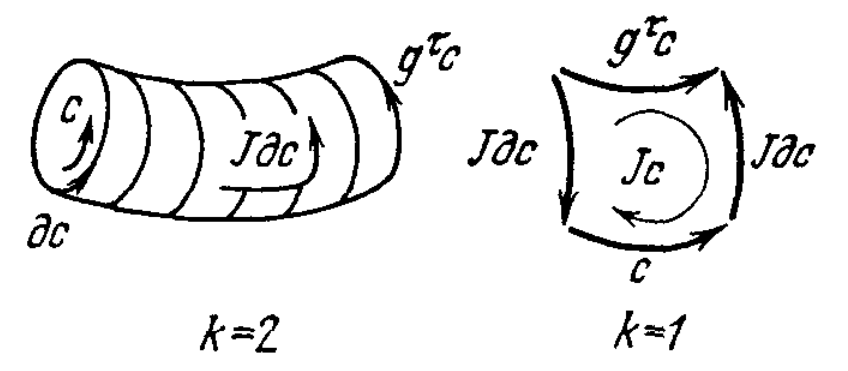
\includegraphics[width=0.3\textwidth]{imgs/chains.png}
    \caption{След цепи при гомотопии}
    \label{fig:сhains}
\end{figure}




\begin{to_thr}[]
    Гамильтонов фазовый поток сохраняет симплектическую структуру $(g^t)^* \omega^2 = \omega^2$. 
    \label{thrA1}
\end{to_thr}


\begin{to_lem}
    Пусть $\gamma$ -- 1-цепь в симплектическом многообразии $(M^{2n}, \omega^2)$. Пусть $g^t$  -- фазовый поток на $M$ с функцией Гамильтона $H$. Тогда
    \begin{equation*}
        \frac{d }{d \tau} \int_{J \gamma} \omega^2 = - \int_{g^\tau \gamma} d H.
    \end{equation*}
\end{to_lem}

\begin{proof}[$\triangle$]
Рассмотрим цепь $\gamma$ из одного куска $f \colon  [0, 1] \mapsto M$, пусть $f'(s, t) = g^t f(s)$, $\xi = \partial_s f'$ и $\eta = \partial_t f' \in TM_{f'(s, t)}$.

По определению интеграла
\begin{equation*}
    \int_{J\gamma} \omega^2 = \int_0^1 \int_0^\tau \omega^2 (\xi, \eta) \d t \d s
\end{equation*}
Но, по определению фазового потока $\eta$ -- вектор гамильтонова поля в точке $f'$, и снова по определению гамильтонова поля $\omega^2 (\eta, \xi) = \d H(\xi)$, тогда
\begin{equation*}
    \int_{J\gamma} \omega^2 = - \int_0^\tau \left(
        \int_{g^t \gamma}  \d H
    \right) \d \tau.
\end{equation*}
\end{proof}

Как некоторое следствие, можно выделить, что если $\gamma$ замкнута ($\partial \gamma =0$), то $\int_{J\gamma} \omega^2 = 0$, по теореме Стокса: $\int_\gamma \d H = \int_{\partial \gamma} H = 0$. 

\begin{proof}[$\triangle$оказательство теоремы]
    Рассмотрим некоторую 2-цепь, тогда для неё
    \begin{equation*}
        0 
        \overset{(1)}{=} 
        \int_{Jc} \d \omega^2 
        \overset{(2)}{=}
        \int_{\partial Jc} \omega^2 
        \overset{(3)}{=} 
        \int_{g^\tau c} - \int_c - \int_{J \partial c} \omega^2 
        \overset{(4)}{=} 
        \int_{g^\tau c}^{} \omega^2 - \int_c \omega^2,
    \end{equation*}
    где $(1)$ равенство верно по замкнутости $\omega^2$, второе по формуле Стокса, третье -- расписали границу цепи, и последнее по предыдущему следствию. 
\end{proof}

% \begin{equation*}
%     \frac{\partial^2 L}{\partial \dot{q}^i \dot{q}^j} = 
%     \frac{\partial p_j}{\partial \dot{q}^i},
%     \hspace{5 mm} 
%     \det\left(
%         \frac{\partial^2 L}{\partial \dot{q}^i \dot{q}^j} 
%     \right) = 0 = 
%     \det \left(
%         \frac{\partial p_j}{\partial \dot{q}^i}
%     \right)
% \end{equation*}



\begin{to_def}
    Дифференциальная $k$-форма $\omega$ называется \textit{интегральным инвариантом} отображения $g$, если интегралы $\omega$ по любой $k$-мерной цепи $c$ и по её образу при отображении $g$ одинаковы: $\int_{g[c]} \omega = \int_x \omega$. 
\end{to_def}



\begin{to_thr}[аналог thr \ref{thrA1}]
    Задающая симплектическую структуру форма $\omega^2$ является интегральным инвариантом гамильтонова фазового потока. 
\end{to_thr}


Также $(\omega^2)^2 = \omega^2 \wedge \omega^2$, и друге <<степени>> являются интегральными инвариантами фазового потока. 

\begin{to_def}
    Отображение $g \colon  \mathbb{R}^{2n} \mapsto \mathbb{R}^{2n}$ называется \textit{каноническим}, если оно имеет $\omega^2$ интегральным инвариантом. Каждая из форм $\omega^4$, $\omega^6$, ..., $\omega^{2n}$ является интегральным инвариантом всякого канонического отображения. Следовательно, при каноническом отображении сохраняется сумма ориентированных площадей проекций на координтные плоскости $(p_i,\, q^j)$. В частности, \textit{канонические отображения сохраняют объёмы}. 
\end{to_def}


\begin{to_def}
    Дифференциальная $k$-форма $\omega$ называется \textit{относительным интегральным инвариантом} отображения $g \colon  M \mapsto M$, если $\int_{gc} \omega = \int_c\omega$ для всякой \textit{замкнутой} $k$-цепи $c$. 
\end{to_def}


\begin{to_thr}[]
    Пусть $\omega$ -- относительный интегральный инвариант отображения $g$, тогда $d \omega$ -- абсолютный абсолютный интегральный инвариант $g$. 
\end{to_thr}

\begin{proof}[$\triangle$]
 Пусть $c$ это $k+1$-цепь, тогда
 \begin{equation*}
     \int_c d \omega = \int_{\partial c} \omega = \int_{g \partial c} \omega = \int_{g c} d \omega.
 \end{equation*}
\end{proof}



Например, каноническое отображение имеет относительный интегральный инвариант $\omega^1 = \vc{p} \d \vc{q} = p_i \d q^i$. 


\begin{to_thr}[закон сохранения энергии]
    Функция $H$ является первым интегралом гамильтонова фазового потока с функцией Гамильтона $H$. 
\end{to_thr}

\begin{proof}[$\triangle$]
Производная $H$ по направлению $\eta$ равна значению $\d H$ на $\eta$. Тогда, по определению
\begin{equation*}
    \d H (\eta) = \omega^2 (\eta,  I \d H) = \omega^2 (\eta, \eta) = 0.
\end{equation*}
\end{proof}



\subsubsection*{Алгебра Ли векторных полей}


\begin{to_def}
    \textit{Алгеброй Ли} называется линейной пространство $L$ вместе с билинейной кососимметричной операцией (\textit{коммутатором}) $L \times  L \mapsto L$, удовлетворяющей тождеству Якоби
    \begin{equation*}
        \left[[A, B], C\right] + \left[[B, C], A\right] + \left[C, A], B\right] = 0.
    \end{equation*}
\end{to_def}


Со всяким гладким полем на многообразии связаны следуюшие два объекта: \vspace{-2mm}
\begin{enumerate*}
    \item \textit{Однопараметрическая группа диффеоморфизмов}, или \textit{поток} $A^t \colon  M \mapsto M$, для которого $\vc{A}$ -- поле скоростей:
    $d_t |_{t=0} A^t (x) = \vc{A}(x)$.
    \item \textit{Производная по направленю} поля $\vc{A}$: дял всякой функции $\varphi M \mapsto \mathbb{R}$ \textit{производная по направлению} $\vc{A}$ есть $L_{\smallvc{A}} \varphi $ такая, что $(L_{\smallvc{A}}\varphi )(x) = d_t |_{t=0} \varphi(A^t x)$.
\end{enumerate*}


Вполне естественно ввести коммутатор дифференцирования по направлениям $\vc{A}$ и $\vc{B}$:
\begin{equation*}
    \frac{\partial^2}{\partial s \ \partial t} \bigg|_{t=s=0} \varphi(A^t B^s x) - \varphi(B^s A^t x) = \left(
        L_{\smallvc{B}} L_{\smallvc{A}} - L_{\smallvc{A}} L_{\smallvc{B}} \varphi
    \right) (x),
\end{equation*}
где возникший коммутатор -- дифференциальный оператор первого порядка, который соответсвует некотором векторному полю $\vc{C}$.


\begin{to_def}
    \textit{Скобкой Пуассона} или \textit{коммутатором} двух векторных полей $\vc{A}$ и $\vc{B}$ на многообразии $M$ называется векторное поле $C$, для которого
    \begin{equation*}
        \li{C} = \li{B} \li{A} - \li{A} \li{B}, \hspace{5 mm} \vc{C} = [\vc{A}, \vc{B}],
    \end{equation*}
    или, в компонентах:
    \begin{equation*}
        [\vc{A}, \vc{B}]^j = 
        B^i \partial_i A^j - A^i \partial_i B^j.
    \end{equation*}
\end{to_def} 

\begin{to_thr}[]
    Скобка Пуассона превращает линейное пространство векторных полей на многообразии $M$ в алгебру Ли, в частности  выполняется тождество Якоби. 
\end{to_thr}

\begin{to_thr}[]
    Два потока $A^t$ и $B^s$ коммутируют тогда и тоько тогда, когда скобка Пуассона соответсвующих векторных полей $[\vc{A}, \vc{B}]$ равна нулю. 
\end{to_thr}





\subsubsection*{Алгебра Ли функций Гамильтона}


Вернемся к симплектическому многообразию, функции $H \colon  M^{2n} \mapsto \mathbb{R}$ заданной на многообразие, и соответствующей однопараметрической группе $g_H^t \colon  M^{2n} \mapsto M^{2n}$ канонических преобразований, $M^{2n}$ -- фазовый поток с функцией гамильтона $H$. Пусть $F \colon  M^{2n} \mapsto \mathbb{R}$ -- другая функция на многообразии $M^{2n}$.

\begin{to_def}
    Скобкой Пуассона $\left\{F,\, H\right\}$ функций $F$ и $H$, заданных на симплектическом многообразии, называется производная функции $F$ по направлению фазового потока с функцией $H$:
    \begin{equation*}
        \{F, H\} (x) = \frac{d }{d t} \bigg|_{t=0} F(g^t_H (x)).
    \end{equation*}
\end{to_def}

\begin{to_con}
    Функция $F$ тогда и только тогда является первым интегралом фазового потка с функцией Гамильтона $H$, когда её скобка Пуассона с $H$ равна нулю: $\{F,\, H\} \equiv 0$.
\end{to_con}


Если вспомним про изоморфизм $I$ между 1-формами и векторными полями  вида $\omega^2 (\eta,\, I \omega^1) = \omega^1 (\eta)$. Вектор скорости фазового потока $g_H^t = I \d H$.

Скобка Пуассона функций $F$ и $H$ равна равна значению 1-формы $\d F$ на векторе $I \d H$ скорости фазового потка с функцией Гамильтона $H$:
\begin{equation*}
    \{F,\, H\} = \d F (I\d H) = 
    \omega^2(I \d H, I \d F),
\end{equation*}
откуда очевидно, что скобка Пуассона кососимметрическая билинейная функция. Тогда можем обобщить теорему Э. Нётер:

\begin{to_thr}[]
    Если функция Гамильтона $H$ выдерживает группу канонических преобразований, заданную гамильтонианом $F$, то $F$ есть первый интеграл системы с функцией Гамильтона $H$. 
\end{to_thr}

Стоит заметит, что в координатах $\{F,\, H\} = \left[
    I \d H,\, I \d F
\right] = \[\grad H,\, \grad F\] = \partial_{p_i} H \partial_{q^i} F - 
\partial_{q^i} H \partial_{p_i}F$. Также стоит вспомнить, что в базисе $(\vc{p},\, \vc{q})$ $I$ имеет вид 
\begin{equation*}
    \begin{pmatrix}
        0 & -E \\
        E & 0
    \end{pmatrix}.
\end{equation*}